\title{N-Graph Abstraction}
\author{
  Cameron W.
 Smith and Gerrett Diamond\\
}
\date{\today}

\documentclass[12pt]{article}
\usepackage{hyperref}
\usepackage{graphicx}
\begin{document}
\maketitle

\section{Overview} \label{overview}
EnGPar interfaces to the (hyper)graph, geometric, and diffusive dynamic
partitioning procedures through the N-Graph abstraction.  

Towards supporting the effective execution of a combination of (hyper)graph,
geometric and diffusive partitioning methods on both graph and mesh data the
N-graph is defined as $G^n(V,E_0,E_1,...,E_{n-1})$ where:
\begin{itemize}
  \item $V$ atomic units $u_i$ of the domain $\omega$ which uniquely exist on one
    part such that $\omega = \bigcup_{\forall_i}u_i$, and 
  \item $E_i$ relations $e_i(u,v)$ of type $i$ between vertices $u$ and $v$
    where $u,v \in V$.
\end{itemize}
Optionally, vertices and edges may be assigned associated weights $w$.  
Vertices may also have a spatial relation in the form of a coordinate vector $c$.
Coordinates define a spational relation but don't necessarily have to be of $d$
dimensions for a $d$-dimension domain.
For example, projecting a set of points to a $d+1$ dimension unit
sphere\cite{gilbertGeo,kirmani2013scalable}.

Applications mapping to this abstraction will define atomic domain entities as
vertices in the N-graph and at least one relation between them.
In this manner applications may represent multiple relations of different
sparsity and degree.
For example the topology of an unstructured 3D mesh may be represented via
vertices defined as mesh elements, and an edge type for each entity shared by
adjacent elements.
Additionally, applications can map to the abstraction at multiple different data
granularity levels to define a sequence of partitioning operations that operate
hierarchically~\cite{turka2012code}.
Completing the N-Graph design documentation will be a year one development in
the research program.

Leveraging this abstraction is the N-Graph Partitioner, EnGPar.
As applications map relations to edge types and define vertex spatial
coordinates EnGPar provides access to partitioning methods.
For instance, with spatial coordinates and one vertex relation defined EnGPar
supports (hyper)graph-based multilevel k-way, recursive inertial(coordinate)
bisection~\cite{williamsRIB}, and multi-criteria iterative
diffusive~\cite{Smith2015}.
Figure~\ref{fig:meshMapping} depicts the mapping of an unstructured mesh (a) to
a representation that supports Vertex$>$Element (b) and Vertex=Edge$>$Element
balancing in (c).
Here the N-Graph vertices represent the mesh elements with one edge type added
for element vertices, as shown in (b), and a second edge type added for mesh
edges in (c).
For simplicity, Figure~\ref{fig:meshMapping} depicts multiple edges with the same
type and bounding vertices by the set of mesh entities they represent.
For example the edge labeled $M^0_{4,1}$ between  $M^2_0$ and $M^2_1$ represents
two edges in the N-Graph; one for the shared vertex  $M^0_4$ and another for
$M^0_1$.
The mesh vertices bounding only a single element are depicted as a loop. 

\begin{figure}
  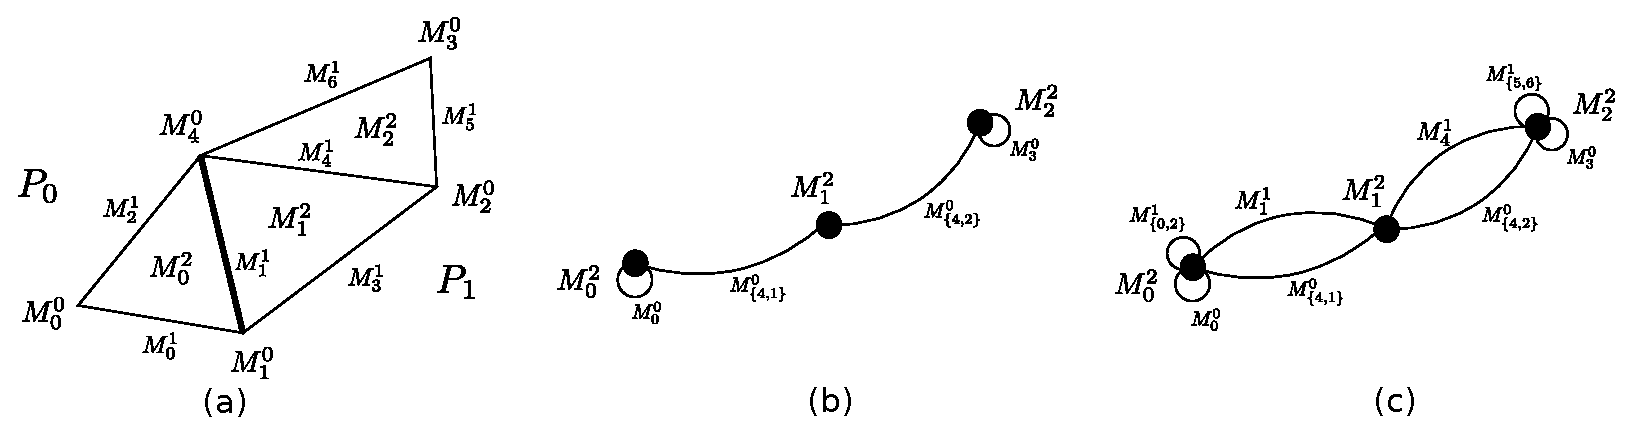
\includegraphics[width=\textwidth]{meshToNgraph.eps}
  \caption{\label{fig:meshMapping}
    Mapping of an unstructured mesh (a) to the N-Graph abstraction for vtx$>$elm
    (b) and vtx=edge$>$elm balancing (c).
  }
\end{figure}

Applications control the partitioning quality via an application defined
priority list of relations to balance and their precedence relative to vertex
imbalance.
For example if an unstructured mesh based linear finite element code defines
vertices as mesh elements and shared element vertices via relation $E_0$, the
balance of $E_0$ could be defined to take precedence over the balance of
vertices to improve the scaling of the solve at the expense of increasing the
imbalance during matrix
assembly~\cite{Zhou2010,rasquinCise2014,zhou2012unstructured,zhou2012tools}.
For each relation the target imbalance level is also specified.

Given the N-Graph, the priority list and target imbalance levels EnGPar supports
partitioning methods to optimize runtime, memory usage, energy efficiency, or
paritition quality.
\begin{itemize}
  \item Applications using explicit solvers which require frequent balancing,
    but cannot afford the computational expense of optimal partition quality,
    benefit from methods that are fast and minimize data movement.
  \item Application using implicit solvers and less frequent adaptive cycles
    have a net benefit from optimal partitional quality at the expense of
    increased runtime or memory usage.
  \item Applications with an adaptive procedure operating at the limits of
    available memory require load balancing that minimizes memory consumption at
    the expense of partition quality and runtime.
  \item Workflows requiring large initial partitions can reduce energy usage by
    performing the multiple intermediate partitionings in-memory and avoiding
    file I/O. See section~\ref{sec:later}.
\end{itemize}


\subsection{Interface Design}

Critical to the efficient design of EnGPar are functional interfaces to
applications that abstract the underlying data structures.
EnGPar minimizes the number of application data transformations by providing
applications a small set of functions to implement.
At the core of the interface are the vertex and edge representations.
To support dynamic partitioning the distribution of the N-graph across memory
domains is queried through the Part object.
A possible interface to EngPar N-graph is defined by the following procedures:

\begin{verbatim}
Vertex
// get the weight of u
real weight(vtx u); 
// get the part id of u
integer partId(vtx u); 
// get the coordinates of u
vector<real> coordinates(vtx u);
// get edges of type t incident to u
list<edges> edges(vtx u, etype t); 
Edge


// get the weight of e
real weight(edge e); 
// get the vtx of e
vtx u(edge e);
vtx v(edge e); 
// get the other vtx of e
vtx other(edge e, vtx u);
Part


// create a vtx iterator 
vtxItr createItr(part p); 
// advance iterator
vtx next(vtxItr itr);
// destroy the iterator itr
destroyItr(vtxItr itr);
// get part id of p
integer partId(part p);
// get |V| | u ϵ V,p 
integer numVtx(part p);
// get |Et| | e(u,v) ϵ Et, u ∨ v ϵ p 
integer numEdges(part p, etype t);
Utility


// determine if two vtx are the same
boolean isEqual(vtx u, vtx v); 
// migrate vtx to target parts
migrate(map<vtx, integer> m);
\end{verbatim}

The vertex equality functions support counting the degree of connectivity
between two vertices needed by the diffusive vertex selection
metrics~\cite{Fiduccia1982,Kernighan1970}.
For example, the number of vertices shared by two triangular mesh faces with a
shared edge on the part boundary can be found by counting the number of edges
bounded by the same vertices.
A migration function is defined to support diffusive methods that require
executing several migration rounds before returning control back to the user.
The first version of the N-Graph interface specification and corresponding
user’s guide will be completed in year one of the research program.
As applications are developed and experience grows the specification and guide
will be updated accordingly.

\section{EnGPar Method Implementation} \label{sec:methods}

Applications implement N-Graph interface functions by deriving the N-Graph base
class.
Polymorphism enables EnGPar partitioning methods and interfacing to third-party
partitioning methods to be implemented without direct knowledge of the
applications underlying data structures.
Zoltan2’s interface design uses a similar approach but is targeted directly for
matrices, array data, and meshes~\cite{zoltan2}.
As part of this research program the N-Graph class would be defined as a fourth
adapter in year two.

Multi-level (hyper)graph methods and geometric methods will be directly
supported by EnGPar as the N-Graph abstraction and it’s APIs are a super-set of
the (hyper)graph and geometric relational abstractions.
The following sub-sections discuss the planned EnGPar implementation of two
ParMA procedures.

\subsection{Multi-criteria Diffusive Improvement} \label{sec:diffusion}

The following pseudo code outlines the process using the N-graph interface to
select vertices for migration from part the local part to neighboring lightly
loaded parts such that the imbalance of higher priority edge type et is not
degraded.
Vertices on the part boundary with more inter-part edges than intra-part edges
are selected if there is a neighboring part that shares the vertex, has fewer
vertices than the local part, and has fewer edges of type et than the part with
the most et edges.
Following this selection of vertices, the ‘plan’ map, the N-graph migration
function is run.

\begin{verbatim}
// et (in) high priority edge type
// maxW (in) desired part weight
// plan (inOut) vertices and their destination part ids
SelectVtxForMigration(etype et, real maxW, map<vtx, integer> plan) 
  real vW = sumVtxWeight(…);
  map<integer, real> neighborVtxW = exchangeWeight(vW);
  real etW = sumEdgeWeight(…);
  real maxEtW = getMaxEtWeight(etW);
  vtxItr itr = createItr();
  while ( vtx u = next(itr) ) {
    if( vWeight - weight(plan) <  maxW ) break; // enough vertices selected
    list<edges> E = edges(u,et);
    integer in = countInternal(E); // intra-part edges internal to the part
    integer ext = E.size() – in; // inter-part edges
    if ( ext <= in ) continue; // low gain 
    // determine if there is a neighboring part that is a candidate
    for ( e in E ) {
      vtx v = other(e, v);
      if ( neighborVtxW.has(v) && vw > neighborVtxW[v] && etW < maxEtW ) {
         plan[vtx] = targetPartId;
         break;
      }
    }
  }
  destroyItr(itr);
}
\end{verbatim}

\subsection{Merge-Split Improvement} \label{sec:msi}

Merge-Split Improvement (MSI) uses the N-graph interface to quickly reduce the
imbalance in a heavily imbalanced partition.
MSI begins by merging neighboring lightly loaded parts to create empty parts.
It then splits the heaviest parts into the empties. Clearly, an optimal
solution is one that produces the greatest reduction in the peak imbalance.
Obtaining this solution requires determining which of the heaviest parts can be
split, and thus their post-split size, given a maximum allowed size of the
merged parts.
Since the merged parts size can be estimated without changing the partition by
summing the weights of the to-be-merged parts, a search for the optimal maximum
merge part size can be performed with minimal expense relative to the
modification of the partition.
Computation of the possible merging combinations for each lightly loaded part
is through each parts solution of the 0-1 Knapsack problem where the capacity
is the allowed merged part size, the items to be selected are the parts (the
local part and its neighbors), the item weight is the sum of the vertex
weights, and the item value is one.
The selection of which merges will be performed such that there are no merging
conflicts, each part can be merged into at most one part, is through Luby’s
maximal independent set~\cite{luby1985simple}.
Both Luby’s algorithm and a dynamic programming algorithm to solve knapsack
only require N-Graph’s interface functions to iterate over part vertices and
query their weight, and neighborhood communication procedures like those
provided by PCU~\cite{ibanez2014hybrid}.

\section{Method Selection} \label{sec:methodSelection}

EnGPar methods are selected based on the applications priority list, the
quality of the input partition, and the number of processors being used.
For example, if the input partition has over 32 thousand parts and an imbalance
of over 100\% MSI improvement can be first applied followed by multi-criteria
diffusive improvement.
If there are fewer parts then either a geometric or (hyper)graph method can be
ran instead of MSI.
As methods are added to EnGPar in years two and three of the research program
the logic controlling their automated selection will be incorporated.
Consideration will be given to incorporating libraries such as
HWLOC~\cite{broquedis2010hwloc} and MonEQ~\cite{wallace2013measuring} to drive
method selection towards those that avoid hardware bottlenecks or energy
intensive communication paths.


INSERT FLOW CHART FROM PHASTA-PARMA PAPER

\section{Application Support} \label{sec:apps}

Three demonstration application areas will be addressed.
The first will be to meet additional needs of adaptive unstructured mesh
simulations not currently met by ParMA The second will be multimodel/big data
applications associated with multiscale materials modeling.
The third will provide dynamic load balancing for massive scale-free graphs
that can be applied in big data applications such as modeling social networks,
or web activities.
Demonstrations will be run on AMOS, the one petaflop RPI IBM Blue Gene/Q, Mira,
the 10 petaflop IBM Blue Gene/Q, and other systems as they become available.
Dynamic Load Balancing for Adaptive Mesh-Based Simulation Workflows In-memory
adaptive unstructured mesh CFD analysis performed with the combination of
PUMI, and PHASTA will be coupled to EnGPar in years one and two for initial S
to T partitioning, multi-criteria load balancing, and predictive load balancing
for mesh adaptation.

S-T partitioning: Although leadership class parallel systems have proportionally
capable file systems, the time spent in file i/o for intermediate partition stages
is orders of magnitudes more expensive than mesh generation and partitioning.
To avoid file i/o costs, and reduce the time to compute the T partition,
compute resources are over allocated such that partitioning stages can all be
performed in-memory.
Following this approach, parallel mesh generation to S parts run on S processes
of a compute allocation supporting T processes is followed by successive
partitioning operations until the target partition size of T is reached.
As part of this research program the energy costs of this in-memory approach,
and the classic file i/o based approach will be analyzed to determine the
potential for net energy savings on the IBM BlueGene /Q via the MonEQ APIs
~\cite{wallace2013measuring}.

EnGPar will support in-memory S-T partitioning by operating on a PCU
sub-communicator associated with each partitioning stage.
Intermediate partitions will target the inter-node concurrency levels through
application of a Zoltan global (hyper)graph and geometric methods while the
final partitioning stage will target the intra-node concurrency level with a
local (hyper)graph method that keeps topologically adjacent parts within the
same NUMA domain.
Multi-criteria load balancing will be applied to this partition to target
application specific requirements.

Multi criteria load balancing: Critical to PDE analysis code scalability is
having minimal element imbalance for matrix formation and minimal imbalance of
degree of freedom holders during equation solution.
EnGPar’s multi-criteria partition improvement methods, derived from ParMA
methods, will support the effective creation of this partition.
The application of these methods will also be demonstrated with a general
high-order unstructured mesh analysis code (e.g.,
Nektar++~\cite{Cantwell2015205}) where there can be different numbers of degrees
of freedom associated with all orders (vertex, edge face and regions) of mesh
entities~\cite{shephard1997straightforward}.

Predictive load balancing: Mesh adaptation driven by anisotropic error
indicators that significantly change the mesh size can result in the possible
failure of mesh adaptation due to exhaustion of available memory.
Memory usage will be controlled by invoking EnGPar’s MSI and diffusive
improvement methods within MeshAdapt using N-Graph weights estimating mesh
density changes.

\subsection{Dynamic Load Balancing for Evolving Multimodel Simulation Workflows}
Multimodel problems introduce new challenges that require multilevel load
balancing The first multimodel problem to be considered is the hierarchic
multiscale modeling of soft tissue~\cite{luo07} using the AMSI multiscale
simulation infrastructure~\cite{del09}.
In this two scale model a microscale model is updated on every macro-increment
at points in each element in an adapting macroscale mesh.
The micro model executed at each of these points to provide local macro model
material properties is either a constitutive model evaluation, a non-linear
fiber network, a non-linear fiber network in parallel with a matrix, or a fully
coupled fiber/matrix representative volume.
Note that the effort required for the different material points evaluations
ranges from a small number of operations, to solving for a full load increment
on a non-linear finite element model that must be executed in parallel on a
reasonable number of processes Strategies must be defined and implemented that
can deal with the parallelization of the macromodel, the distribution of the
many micromodels and the parallelization of some of the individual micromodels.
In addition to the complications introduced by doing this as the macro mesh
and selected micromodels are adapted, it should be noted that the micromodels
are themselves non-linear, and experience shows that the number of Newton
iterations needed in any individual increment varies, thus it is not possible
to gain accurate a priori estimates of the cost of the solution of individual
micromodels.
The EnGPar interface to Zoltan will support the hierarchic application of a
local Zoltan method to the micromodels and a global method to the macromodel
Improvement of the micro and macro partitions in response to adaptive changes
will be supported by weighted multi-criteria improvement.
In addition to accounting for macro mesh modifications, the macro improvement
will account for heterogeneous computation loads associated with micro-coupling
through additional weighted N-Graph edges.

A second multiscale problem to be considered will be an adaptive concurrent
atomistic continuum model where molecular dynamics models are applied over a
small portion of the domain, continuum models over the majority of the domain
and both model, and their interaction, solved in small overlap region between
the two.
EnGPar MSI and diffusive improvement will be regularly applied to ensure even
computational load distribution of the two models and control model to model
communication in the overlap region as the size and shape of the atomic region
is adapted.
Interactions with AMSI developers in year two will be critical to the analysis
of partition characteristics and the subsequent design, development and testing
of inexpensive balancing procedures.

\subsection{Dynamic Load Balancing for Evolving Discrete Event Simulations} 
Constantly evolving massive scale-free graphs, such as those modeling social
networks~\cite{twitter2010,kwak2010twitter}, or the world wide web, require
periodic dynamic load balancing to maintain efficient execution of parallel
discrete event simulations~\cite{carothers2002ross}.
As vertex partitionings of scale-free graphs are known to have low quality
~\cite{abou2006multilevel,lang2004finding,leskovec2009community,pienta2013parallel} the feasibility of splitting the communication and computation
load of high degree vertices via a split-vertex dynamic partitioning will be
evaluated as part of this research program.
Towards this, in year three, the N-Graph interface will be implemented such
that the top few percent of high degree graph vertices, d(u) > εMax(d(u)), are
split and represented by log2(d(u))-1 additional N-Graph vertices and edges, as
depicted in Figure~\ref{fig:vtxSplitting}.
A split-vertex partitioning of the source graph prioritizing the imbalance of
edges over vertices is computed using EnGPar’s multicriteria partitioning
methods.
The graph will then be augmented with additional vertices and edges,
maintaining the original distribution characteristics, and the dynamic
partitioning re-applied.
The quality of the partitionings will be evaluated by executing the massively
parallel ROSS~\cite{carothers2002ross,mubarak2012modeling,barnes2013warp}
open-source discrete event simulation engine for modeling computer network virus
propagation.
Through on-going collaborations with Professor Chris Carothers, the principal
author of ROSS, a message passing based shared state update of split vertices
using a scatter/gather update
protocol~\cite{gonzalez2012powergraph,sahni2009scalable} as depicted in
Figure~\ref{fig:vtxSplitting} will be integrated into ROSS.

\begin{figure}
  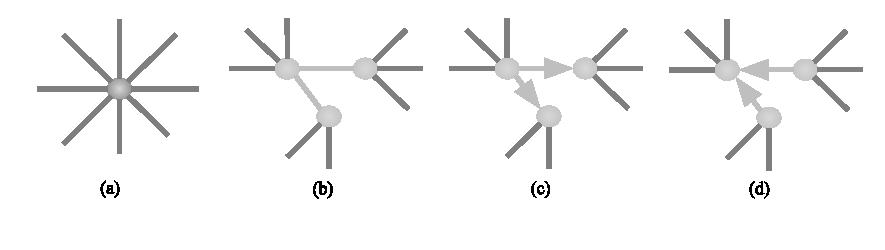
\includegraphics[width=\textwidth]{vtxSplitting.eps}
  \caption{\label{fig:vtxSplitting}
    High degree vertex splitting. 
    The original high degree vertex in (a), the split N-graph representation in
    (b), and the scatter and gather update protocol in (c) and (d) respectively.
  }
\end{figure}

\bibliographystyle{plain}
\bibliography{references}

\end{document}
